\begin{table*}[htbp]
  \centering
  	\caption{Subjects used in our evaluation}
  	%\vspace{-8pt}    
    \begin{tabular}{|l|r|r|r|}
    \hline
    %	\multirow{2}{*}{Subjects} & \multirow{2}{*}{LOC} & \multirow{2}{*}{\# Test Cases} & \multirow{2}{*}{ \# Security Test Cases}  \\\cline{5-7}
    Subject & LOC & \# Test Cases & \# Security Test Cases \\\hline\hline
    LMS   & 3749  & 46    & 29     \\\hline
    VMS   & 3734  & 52    & 10     \\\hline
    ASMS  & 7836  & 93    & 91     \\\hline\hline
    Average & 5106  & 64    & 43     \\\hline
		\end{tabular}%
  \label{tab:subj}%
%\end{table}%
%
%\begin{table*}[tbp]

\vspace{+10pt}
\centering
  \caption{Policy statistics used in our subjects}
  	%\vspace{-8pt}   
    \begin{tabular}{|l|r|r|r|r||r||r|r|r|}
 		\hline
 		     \multirow{2}{*}{Subject} & \multicolumn{4}{|c||}{Attributes} & \multirow{2}{*}{\# Rules} & \multicolumn{3}{|c|}{Policy Coverage}  \\\cline{2-5}\cline{7-9}
 		     
     & ~\# Sub~ & ~\# Act~ & ~\# Res~ & ~\# Cond~ & & \# Cov & \# Not-Cov& \% Cov \\\hline\hline
    LMS   & 6     & 10    & 3     & 4     & 42    & 42    & 0     & 100 \\\hline
    VMS   & 7     & 15    & 3     & 3     & 106   & 13    & 106   & 12 \\\hline
    ASMS~  & 8     & 11    & 5     & 4     & 129   & 109   & 21    & 83 \\\hline\hline
 		Average & 7     & 12    & 4     & 4     & 93    & 55    & 42    & 65 \\\hline

    \end{tabular}%
  \label{tab:subjectpolicies}%
\end{table*}%

%  \centering
%  \caption{Policy statistics used in our subjects}
%  	\vspace{-8pt}   
%    \begin{tabular}{|l|r|r|r|r||r|r|r|}
% 		\hline
% 		     \multirow{2}{*}{Subject} & \multicolumn{4}{|c||}{Attributes} & \multicolumn{3}{|c|}{\# Policy Rules} \\\cline{2-8}
% 		     
%     & ~\# Subjects~ & ~\# Actions~ & ~\# Resources~ & ~\# Conditions~ & ~\# Explicit~ & ~\# Implicit~ & ~\# Total~ \\\hline\hline
%    LMS   & 6     & 10    & 3     & 4     & 42    & 678   & 720 \\\hline
%    VMS   & 7     & 15    & 3     & 3     & 106   & 839   & 945 \\\hline
%    ASMS~  & 8     & 11    & 5     & 4     & 129   & 1631  & 1760 \\\hline\hline
% 		Average & 7     & 12    & 4     & 4     & 93    & 1049  & 1142 \\\hline
%
%    \end{tabular}%
%  \label{tab:subjectpolicies}%
%\end{table*}%


\section{Experiments}\label{sec:experiment}


This section presents the experiments that we conducted to evaluate our proposed
selection and augmentation techniques of regression system tests for policy
evolution. We carried out our evaluation on a PC, running Windows 7 with Intel Core i5, 2410 Mhz processor, and 4 GB of RAM. 
Given a program code interacting with a policy $P$, the regression simulator implements its modified
policy $P'$ by changing/adding/removing random rules in $P$. Our test-selection techniques select test cases that may reveal different behaviors in program code impacted
by policy changes between $P$ and $P$'. We measure effectiveness and efficiency of our test selection techniques in terms of the number of selected 
test cases and elapsed time, respectively. We then apply our proposed test-augmentation technique to generate additional test cases
for augmentation. In this section, we first describe the subjects, objectives, measures, and instrumentation. We next present and discuss the evaluation results
and finally describe threats to validity.


\subsection{Subjects}

We collected three real-life Java programs \cite{mouelhi09:tranforming} each
interacting with policies written in XACML.
These policies are based on OrBAC policy model
illustrated as the example policy in Figure~\ref{fig:example}.
Given a policy, 
Sun's PDP \cite{sun05:xacml} is
used to load a policy and evaluate requests issued from test cases in the programs.
From our three subjects,
Library Management System (\CodeIn{LMS}) provides web services to borrow/return/manage books in a library.
Virtual Meeting System (\CodeIn{VMS}) provides web conference services to organize online meetings.
Auction Sale Management System (\CodeIn{ASMS}) provides web services to manage online auction.
A seller initiates an auction by submitting a description of an item she/he would like to sell with its expected minimum price. Users then participate in bidding process by
bidding the item. Before the bidding, users should have enough money in her/his account.

%\begin{itemize}	
%\item Library Management System (LMS) provides web services to borrow/return/manage books in a library.
%\item Virtual Meeting System (VMS) provides for web conference services to organize online meetings.
%\item Auction Sale Management System (ASMS) provides web services to manage online auction.
%A seller initiates an auction by submitting a description of an item she/he would like to sell with its expected minimum price. Users then participate in bidding process by
%bidding the item. Before the bidding, users should have enough money in her/his account.
%\end{itemize}

Table~\ref{tab:subj} summarizes the basic statistics of our subjects.
The first column shows the subject names.
Columns 2-4 show the lines of code, and the numbers of system test cases and security test cases.
Security test cases refer to system test cases that issue at least one request to the PDP.
Table~\ref{tab:subj} shows that our subjects include about 64 system test cases and 43 security
test cases on average.
In particular, \CodeIn{VMS} is equipped with only 10 security system test (out of 52 system test cases), which
is smaller than those of other subjects.
%of security system test cases than other policies.
%Each security system test case issues at least one request.


Table~\ref{tab:subjectpolicies} summarizes the basic statistics of policies used in our subjects.
The first column shows the subject names.
Columns 2-4 show the numbers of subjects, actions, resources, and conditions within attribute column group, respectively.
Column 5 shows the number of rules for each policy.
Columns 6-7 show the numbers of covered rules with test cases, not-covered rules with test cases, and the percentage
of coverage within policy coverage column group, respectively.
The largest policy is related to \CodeIn{ASMS}, which consists of 129 rules.
%\CodeIn{ASMS} consists of the largest number of rules one consists of 129 rules.
For coverage, we measure which rules are
evaluated (i.e., covered) with existing test cases under test.
We observe that \CodeIn{LMS}, \CodeIn{VMS}, and \CodeIn{ASMS}
achieve 100\%, 12\%, and 83\% policy coverage with given test cases, respectively. 
\CodeIn{LMS}, \CodeIn{VMS}, and \CodeIn{ASMS} may represent subjects
with high, low, and medium policy coverage, respectively.
Moreover, while \CodeIn{VMS} consists of 106 rules, \CodeIn{VMS} is equipped with only 10 security system test cases
that result in low policy coverage.


%, rules, implicit
% rules, and total rules for each policy.
%The largest one consists of 129 rules.
%For explicitly specified rules, developers first write rules for denying or permitting access
%explicitly. Implicit rules refer to rules that are evaluated in a given policy, while the developers do not write such rules.
%For example, In Figure~\ref{fig:example}, Line 34
%specifies a rule. This rule denies all the requests $R_d$ that do not match with its preceding rules while
%no rules (i.e., implicit rules) are specified to handle such requests explicitly.
%We observe that \CodeIn{LMS}, \CodeIn{VMS}, and \CodeIn{ASMS}
%achieve 100\%, 12\%, and 83\% policy coverage with given test cases, respectively. 
%\CodeIn{LMS}, \CodeIn{VMS}, and \CodeIn{ASMS} may represent subjects
%with high, low, and medium policy coverage, respectively.
%Moreover, while \CodeIn{VMS} consists of 106 rules, \CodeIn{VMS} is equipped with only 10 security system test cases
%(out of 52 system test cases) that issue at least one request.






% Performing equivalent mutation detection is
%costly, taking approximately 45 minutes for the whole experiment.
%When considering the low percentage of detection, potential for
%false positives, and high computational cost, we feel other means
%of equivalent-mutant detection are needed

%In addition, over all of existing test cases, we distinguish security test cases, which issue
%more than one request to the PDP from test cases without interaction of policies.



%program code, which represents the actual
%functionality, interacts with a policy through a security
%component, called Policy Decision Point (PDP).
%
%Our subjects include 
%
%The PEPs next submit the request to a PDP, which
%evaluates the request against the policy loaded on the PDP
%
%include a separately specified policy loaded with the Sun PDP~\cite{sun05:xacml};
%Sun's PDP is popularly used PDP to evaluate requests against XACML policies.


\begin{table*}[htbp]
  \centering
  \caption{Coverage results of test cases selected for changed policy behaviors for each policy}
  	%\vspace{-8pt}   
    \begin{tabular}{|l|r|r|r||r|r|r||r|r|r||r|r|r||r|r|r|}
%\multirow{2}{*}{Subject} & \multicolumn{3}{c}{Regression - 5} & \multicolumn{3}{c}{Regression - 10} & \multicolumn{3}{c}{Regression - 15} & \multicolumn{3}{c}{Regression - 20} & \multicolumn{3}{c}{Regression - 25} & \\
\hline
     \multirow{2}{*}{Subject} & \multicolumn{3}{|c||}{Regression - 5} & \multicolumn{3}{|c||}{Regression - 10} & \multicolumn{3}{|c||}{Regression - 15} & \multicolumn{3}{|c||}{Regression - 20} & \multicolumn{3}{|c|}{Regression - 25} \\\cline{2-16}
       & \# CT & \# Cov & \% Cov & \# CT & \# Cov & \% Cov & \# CT & \# Cov & \% Cov & \# CT & \# Cov & \% Cov & \# CT & \# Cov & \% Cov \\\hline\hline
    LMS   & 5.0   & 2.4   & 48.3  & 9.0   & 4.8   & 52.8  & 13.0  & 6.3   & 48.1  & 17.4  & 7.8   & 44.5  & 20.7  & 8.8   & 42.7 \\\hline
    VMS   & 4.9   & 0.4   & 8.5   & 9.3   & 0.7   & 7.2   & 13.8  & 1.3   & 9.6   & 18.9  & 1.1   & 5.7   & 23.8  & 1.8   & 7.4 \\\hline
    ASMS  & 5.0   & 1.9   & 38.3  & 9.8   & 4.8   & 48.7  & 14.4  & 7.3   & 50.9  & 18.7  & 9.4   & 50.4  & 23.3  & 12.1  & 51.8 \\\hline\hline
    Average & 4.97  & 1.58  & 31.71 & 9.33  & 3.39  & 36.23 & 13.75 & 4.97  & 36.19 & 18.33 & 6.08  & 33.56 & 22.58 & 7.56  & 33.97 \\\hline

    \end{tabular}%
  \label{tab:cov-results}%
\end{table*}%

%techniques as test selection based on mutation analysis ($Mut-Selection$)
%test selection based on coverage analysis ($Cov-Selection$)
%test selection based on recorded rrequest evaluation ($Req-Selection$)

% Table generated by Excel2LaTeX from sheet 'Performance'
\begin{table*}[htbp]
  \centering
  \caption{Elapsed time for each step of test selection technique, and each policy}
  	%\vspace{-8pt}   
    \begin{tabular}{|l|r|r|r||r|r|r||r|r|}

			\hline
       \multirow{2}{*}{Subject}   & \multicolumn{3}{|c||}{Mut-Selection} & \multicolumn{3}{|c||}{Cov-Selection} & \multicolumn{2}{|c|}{Req-Selection} \\\cline{2-9}

%          & Pre-computed & \multicolumn{2}{c}{Post-computed} & Pre-computed & \multicolumn{2}{c}{Post-computed} & Pre-computed & Post-computed \\\cline{2-7}
          & Rule-Test & CIA & Test Selection & Rule-Test & CIA& Test Selection & Req Collection & Test Selection \\\hline\hline
%    LMS   & 70496 & 2083.333333 & 4.25  & 5214  & 2083.333 & 4.25  & 2096  & 1.933333 \\\hline
%    VMS   & 19771 & 3333.333333 & 0.766667 & 7506  & 3333.333 & 0.766667 & 1873  & 1.866667 \\\hline
%    ASMS  & 118248 & 4000  & 11.36667 & 22423 & 4000  & 11.36667 & 1064  & 20.7 \\\hline

		LMS   & 70496 & 2083  & 4     & 5214  & 2083  & 4     & 2096  & 2 \\\hline
    VMS   & 19771 & 3333  & 1     & 7506  & 3333  & 1     & 1873  & 2 \\\hline
    ASMS  & 118248 & 4000  & 11    & 22423 & 4000  & 11    & 1064  & 21 \\\hline\hline
    Average & 69505 & 3139  & 5     & 11714 & 3139  & 5     & 1678  & 8 \\\hline

    
    \end{tabular}%
  \label{tab:performance-results}%
\end{table*}%

\subsection{Objectives and Measures}
In the evaluation, we intend to address the following research questions:
\begin{itemize}


	\item RQ1: How high percentage of test cases (from an existing test suite) are reduced by our test selection techniques? This question helps to show that our techniques can 
	reduce the cost of regression testing.
%	reduce a significant number of test cases for regression testing.
	We also show how many changed policy behaviors are covered with our selected test cases.
	
%	\item RQ2: Do our protest selections are safe? This question helps to show that our techniques select all tests, which shows only and all test cases to reveal changed behaviors in access control policies.
	
	\item RQ2: How much time do our techniques take to conduct test selection by given subjects? This question helps to compare performance of our techniques by measuring their efficiency.
			
	\item RQ3: How high is the additional policy coverage ratio that is achieved by our test augmentation technique?  This question helps to show that our technique can generate augmented test cases to cover 100\% of changed policy behaviors.
%We also compare our approach with random test generation technique to show how effectively our approach augment test suite to cover not-coverted changed policy behaviors.
				
\end{itemize}

To help answer these questions, we collect few test metrics to show the effectiveness and the efficiency of our test selection techniques and
our test augmentation technique. 
The following metrics are
measured for each subject under test interacting with each modified policy
and each technique.
\begin{itemize}
%	\item \textit{Selected test case count}.  The test count is the size of the request set or
%the number of tests generated by the chosen test-generation
%technique. For testing access control policies, a test is synonymous with request
	\item \textit{Test reduction percentage.}  Given a policy and its modified
	policy, the test reduction percentage is the number of selected test cases for regression testing divided by the number of security test cases.
		\item \textit{Changed policy behavior count.}  Given a policy and its modified
	policy, the changed policy behavior count is the number of impacted rules by policy changes.
	\item \textit{Changed policy behavior coverage count.}  Given a policy and its modified
	policy, the changed policy behavior coverage count is the number of
	impacted rules covered with existing test cases.
	\item \textit{Changed policy behavior coverage percentage.}  Given a policy and its modified
	policy, the changed policy behavior coverage percentage is the changed policy behavior coverage count divided by the total number of impacted rules.
	\item \textit{Elapsed time.}  The elapsed time is time (measured in milliseconds) elapsed for each step during the test selection process.
	\item \textit{Augmented test case count.}  The augmented test case count is the number of augmented test cases by each augmentation type.
	
\end{itemize}
 
%policy under test, each request set, and each mutation operator.
%\subsection{Metrics}
%
%We use following 4 metrics in our evaluation.
%\begin{itemize}
%	\item Policy coverage information for changed policy behaviors.
%	\item Number of test cases reused by the test selection technique.
%	\item Elapsed time of test-rule correlation, change impact analysis, and test selection.
%	\item Number of test cases generated by the test augmentation technique. 
%\end{itemize}

\begin{figure}[htbp]
    \centering
        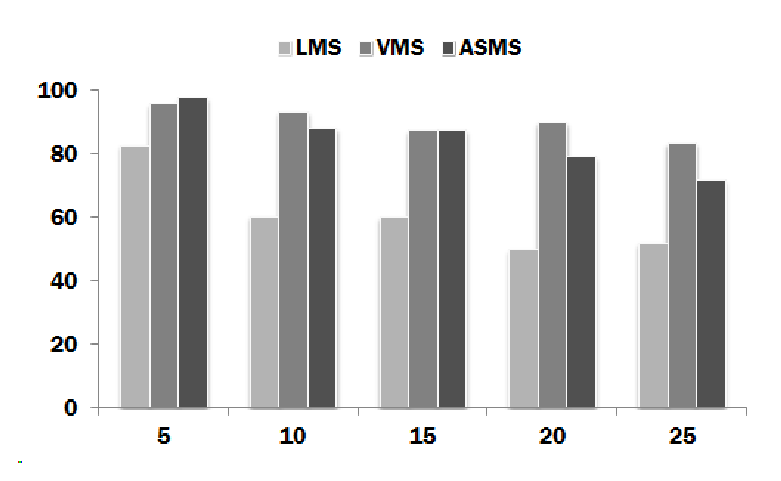
\includegraphics[width=3.0in]{reduction.eps}
        \vspace{-5pt}
    \caption{\label{fig:reduction} Regression test selection results (test reduction) for our subjects and each modified version. Y axis
    denotes the percentage of test reduction. X axis denote the number of policy changes in the modified policy of our subjects.}
    \vspace{-10pt}
%    \vspace{+3pt}
\end{figure}

\subsection{Instrumentation}
For each policy change, the regression simulator first randomly chooses one of regression types from \CodeIn{RMR}, \CodeIn{RA},
and \CodeIn{RDC} and a rule, and changes the rule with a selected type.
We configured the regression simulator to inject 5, 10, 15, 20, and 25 changes in a policy, respectively.
Our evaluation is repeated 12 times in order to avoid the impact of randomness of changes.

For our test selection approach, we use test selection based on mutation analysis ($Mut$-$Selection$),
test selection based on coverage analysis ($Cov$-$Selection$), and
test selection based on recorded request evaluation ($Req$-$Selection$)
described in Section~\ref{sec:approach}.
To measure the effectiveness of our three techniques,
we measure how many test cases are selected for regression testing.

We next compare the efficiency of our three techniques.
The objective of this evaluation is to investigate how our three test selection techniques impact performance. We measure elapsed time to conduct rule-test correlation,
change impact analysis, and test selection for each technique.
For $Mut$-$Selection$ and $Cov$-$Selection$, note that we require rule-test correlation analysis
and change impact analysis, which should be done before actual test selection process.

%To measure the effectiveness of our test augmentation technique,
For test augmentation,
we count the number of new augmented test cases by each augmentation type.

\subsection{Results}
To answer $RQ1$, 
we measure test reduction percentage.
The goal of this research question is to show the reduction in the number of test cases that
are selected using our techniques.
Figure~\ref{fig:reduction} shows the results of test reduction percentage for the three subjects and modified policies.
We observe that our techniques achieve 51\%$\sim$97\% of test reduction for a modified policy with 5$\sim$25 changed policy behaviors.
Such test reduction may reduce a significant cost in terms of test execution time
for regression testing. We also observe that all of our test techniques show the same
set of selected test cases. This observation shows that all of our techniques are
effective to select every test case impacted by policy changes.

Upon further examination
of the results, we find correlation between policy coverage and test reduction.
We notice that \CodeIn{VMS} often shows the highest test reduction compared to \CodeIn{LMS} and \CodeIn{ASMS}.
While the policy $P_{vms}$ used in \CodeIn{VMS} consists of 106 rules, $P_{vms}$ achieves low policy coverage.
$P_{vms}$ achieves only 12\% of policy coverage with 10 security test cases.
This indicates that more than 90 rules are not covered. Due to its low policy coverage, there would be low probability
to find test cases (among existing test cases) for covering impacted rules by policy changes.
On the contrary, the policy $P_{lms}$ used in \CodeIn{LMS} achieves high policy coverage and the lowest
test reduction percentage. Therefore, $P_{lms}$ may find more test
cases to exercise impacted rules than $P_{vms}$. 

 


%The reason is because \CodeIn{VMS} has only 10 security test cases and achieve only 12 policy coverage percentage.
%for 106
%It is difficult to 

%for policy and rule elements, Cirg is at least as good as random
%generation at achieving high structural coverage. We unexpectedly
%notice that Cirg exhibits worse policy and rule coverage than the
%random technique on the mod-fedora policy. Upon further examination
%of that policy we find that two of the policies within the
%policy set are identical. Furthermore, each of these policies contains
%exactly one rule. As a result, there was no change-impact
%when that rule was removed and so Cirg did not generate a request
%to cover that rule or its containing policy.
%We observe that 51\%$\sim$83\% of test reduction for a modified version with 25 policy changes.


To answer $RQ2$, we measure elapsed time.
The goal of this research question is to compare efficiency of our three
test-selection techniques.
Table~\ref{tab:performance-results} shows the evaluation results for the three subjects and
each technique.
For $Mut$-$Selection$ and $Cov$-$Selection$, the table shows the elapsed time of
rule-test correlation (``Rule-Test''), change-impact-analysis (``CIA''), and test
selection (``Test Selection''), respectively.
For $Req$-$Selection$, the table shows the elapsed time of
request recording (``Req-Collection''), and test
selection (``Test Selection'').
Note that ``Rule-Test'' and ``Req-Collection'' are preliminary steps, which
can be done before test selection.
Note that, as both $Mut$-$Selection$ and $Cov$-$Selection$ have the same
change impact analysis step, ``CIA'' column shows the same elapsed
time.
 
We observe that rule-test correlation $TR_1$ of $Cov$-$Selection$ takes
significantly more time than that $TR_2$ of $Mut$-$Selection$.
$TR_1$ and $TR_2$ take 11,714 milliseconds and 69505 milliseconds on average, respectively.
This result is expected as $TR_1$ executes existing test cases only once
but $TR_2$ executes existing test cases for 2$\times$$n$ times where $n$
is the number of rules in a policy under test.
We calculate total elapsed time for each technique. We observe that the total elapsed time of $Req$-$Selection$ is 43 and 8 times
faster than those of $Mut$-$Selection$  and $Cov$-$Selection$, respectively.
As a result, $Req$-$Selection$ is the most efficient
in terms of elapsed time.

%these packet sets can
%involve more structural entities than the other packet sets.
%
%Such results are the same as we expected
%structural
%coverage for the two random request sets is zero and, as expected,
%the mutant-killing ratio is also zero.
%
%takes the highest elapsed time 
%(11,714 milliseconds on average) a significant
%elapsed time compared to $Mut$-$Selection$ (on average 69505 milliseconds) in terms of test-rule correlation.




%$Mut$-$Selection$ and $Cov$-$Selection$ show
%elapsed time 69505 (mm) and 11714 (mm) for test-rule correlation.
% $Cov$-$Selection$  


%the reduction in the number of test cases that
%are selected using our techniques.
%
%To measure the efficiency of our three techniques, we conducted evaluation as follows. 
%We compared elapsed time to analyze test-rule correlation analysis,
%change impact analysis, and test selection by each technique.
%For the first two techniques, we require test-rule correlation analysis
%and change impact analysis, which should be done before actual test selection.
%The objective of this evaluation is to investigate how our three test selection techniques impacts performance for subjects.



Table~\ref{tab:cov-results} shows the coverage results of selected test cases for the three subjects and
the number of changes injected into the policy.
Given a policy $P$,
``Regression - N'' denotes a group of modified policies where $N$ denotes the number of changes injected into $P$. 
For each subject and ``Regression - N'',
the table shows changed policy behavior count (``\# CT''),  changed policy behavior coverage count (``\# Cov''), and changed policy coverage percentage (``\% Cov'').
%changed policy behaviors (``\# CT''), test
%cases that were selected (``\# Cov''), and the percentage of test
%cases that were selected (``\% Cov'') for each version of its policy.
``\# CT'' is equal or less than $N$ because a modified policy may not
reflect some of injected policy changes. The reason is because injected policy
changes may not change policy behaviors semantically.
One example is that policy behaviors do not change
when $RDC$ are injected to the same rule twice.
We observe that the changed policy behavior coverage percentages across all subjects are quite similar. Our techniques achieve 31.71\%$\sim$36.23\% of changed policy behavior coverage percentage.
Unfortunately the
changed policy behavior coverage percentage is still low when considering revealing
faults caused by policy changes.
%changed program behaviors impacted by all of modified policy behaviors.
This observation indicates that test-augmentation
is needed to cover not-covered but impacted rules. 

%the high structural
%coverage.
%
%We observe that 
%As we me

%For example, if $RDC$ are applied to the same rule twice,
%the policy behaviors are 
%
%the same semantically.

%if one changes
%one rule with $RDC$ and again changes the rule with $RDC$.
% may not re
%introduce
%policy behavior changes at the final modified version of the policy.  As the results, the rule does not impact
%on policy changes.



% Table generated by Excel2LaTeX from sheet 'test augument'
\begin{table}[thbp]
  \centering
  \caption{Test case type ratios of augmented test cases for our subjects}
    \begin{tabular}{|l|r|r|r|r|}
		\hline
    Subjects & \% M-Sub & \% M-Cond & \% M-SubCond  & \% M-Others \\\hline\hline
    LMS   & 21.83 & 4.93  & 11.27 & 61.97 \\\hline
    VMS   & 3.41  & 0.38  & 1.89  & 94.32 \\\hline
    ASMS  & 16.30 & 9.63  & 7.41  & 66.67 \\\hline\hline
    Average & 13.85 & 4.98  & 6.86  & 74.32 \\\hline
    \end{tabular}%
  \label{tab:augment-results}%
\end{table}%
 %\vspace{-20pt}
\begin{figure}[htbp]
    \centering
        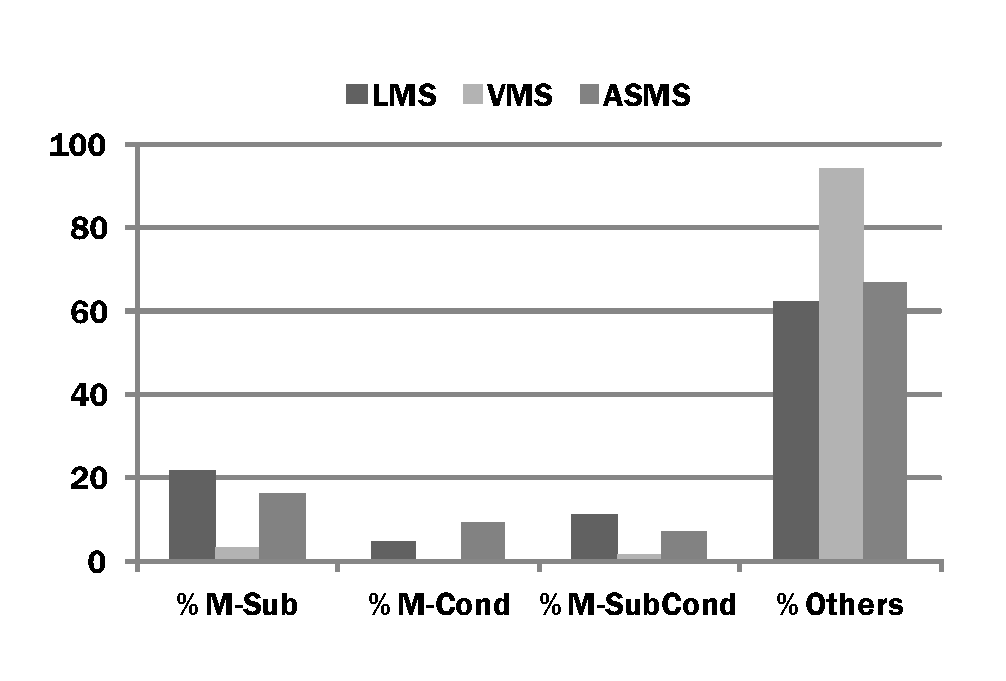
\includegraphics[width=3.0in]{augmenttypes.eps}
        \vspace{-5pt}
    \caption{\label{fig:augment-results} Augmented test results for our subjects and each modified version. Y axis
    denotes the percentage of augmented test cases. X axis denote the types of the augmented test cases.}
    \vspace{-10pt}
%    \vspace{+3pt}
\end{figure}

%[TBD:Results-test augmentation]

To answer $RQ3$, we first identify
not-covered but impacted rules by policy changes
and augment test cases to cover such impacted rules.
%first identify
%changed policy behaviors (i.e., rules impacted by policy changes), which
%are not-covered with existing test cases.
%Note that existing test cases cannot reveal faults introduced by such policy behaviors.
%In Table~\ref{tab:cov-results}, we observe that our selected test cases
%cover 31.71$\sim$36.23\% of changed policy behaviors. The result show
%that about 70\% of changed policy behaviors (i.e., rules impacted by policy changes) are not-covered.
%We apply our test augmentation technique to add new test cases
%to cover such not-covered-rules.
Table~\ref{tab:augment-results} shows the results of test augmentation for the three subjects.
%When developers know which policy behaviors to cover, the developers could generate
%test cases with requests to cover the policy behaviors. 
For each subject, the table shows the percentage of
generated test cases for each augmentation type defined in Section~\ref{subsec:testaugmentation}.
%$[\frac{a}{b}]$ 
While we generate/modify test cases to cover 100\% percentage of not-covered but impacted rules,
``M-Sub'', ``M-Cond'', and ``M-SubCond'' refer to generate test cases by modifying
subject elements, condition elements, and both subject elements and condition elements together, respectively in test cases.
%In our subjects, for these argumentation types, developers can modify existing test cases
%to increase coverage of not-covered but impacted rule. 
``M-Others'' denotes an augmentation type, which
may at least change action and resource elements.
While ``M-Sub'', ``M-Cond'', and ``M-SubCond'' require developers to modify existing
test cases, ``M-Others'' require the developers to create new test cases issuing requests
directly evaluated by the PDP without passing through the PEP. The reason is because the test cases in our subjects are
designed to use variables to define subject elements and condition elements. Therefore,
we achieve our goal by modifying such variables. However, for `M-Others'', we create
new test cases.

\Comment{
we may augment test cases based on following different types of modification/generation.
``M-Sub'' refers to generate test cases by modifying
subject elements in test cases. For example, Given test cases, by changing subject elements (e.g,
BORROWER instead of SECRETARY),
the test cases cover the changed behaviors, which was not-covered in existing test cases
shown in Table~\ref{tab:augment-results}.
Similarly, ``M-Cond'' refers to generate test cases by modifying
condition elements in test cases.
When two of the preceding modification could not
find test cases to modify, our technique finds
``M-SubCond'', which refers to generate test cases by modifying
subject elements and condition elements together.
At the last column, ``M-Others'' denotes an argumentation type, which
may at least change action and resource elements.
}

Table~\ref{tab:augment-results} shows that we achieve
about 26\% (13.85\%+4.98\%+6.86\% on average shown in columns 2,3, and 4, respectively) of the augmented test cases by modifying existing test
cases. However, we generate more than 74\% of the augmented test cases by scratch since we could not find similar
test cases to modify in context of our subjects. Total of each row is 100\%, which indicates that we
generate  augmented test cases to cover 100\% of impacted rules.
Figure~\ref{fig:augment-results} illustrated
the same data shown in Table~\ref{tab:augment-results}.

By comparing these results with those in Table~\ref{tab:cov-results}, we observe that there is indeed a correlation between policy coverage and 
test augmentation type.
The higher percentage of policy coverage for each subject with existing test cases,
the higher percentage of test cases that
are classified to ``M-Sub'', ``M-Cond'', or ``M-SubCond''.
There is high probability that the subject with high policy coverage
finds test cases  for modification than that with low policy coverage.

%fo the subject has test cases with high policy coverage, 
%
%it is likely
%to find similar test cases to modify than subjects with test cases with low rule coverage.

\subsection{Threats to Validity}
The threats to external validity primarily include the degree to
which the subject programs, the policies and regression model are representative of true practice.
These threats
could be reduced by further experimentation on a wider type of policy-based software systems and
larger number of policies.
%composed of any combination of attribute elements.
The threats to internal validity are instrumentation effects
that can bias our results such as faults in Sun's PDP, faults in Margrave, and
faults in our implementation.


\section{Discussion}\label{sec:discussion}
We believe that our approach can be applied to select test cases in programs interacting
with policies written in languages other than XACML.
In practice, many formal specification languages such as EPAL~\cite{epal} and Alloy~\cite{jackson01:micromodularity}
are used to specify policies. 
For those policies written in other languages, we leverage
a PDP that can load the policies to monitor rule-test correlation during running test cases.
As our approach requires change impact analysis step (against a policy and its modified policy) which is handled by 
the existing policy change impact tool, we could convert the policies to XACML policies to perform change impact analysis.

Moreover, our approach relies on changed policy
behaviors (reflected by rules impacted by policy changes) and thus could be applied to other policy models beyond
an OrBAC policy model~\cite{kalam03:orBac}.
While different policy models (such as RBAC~\cite{anderson04:rbacxacml,ferraiolo01:proposed}
and OrBAC) may
be different in terms of structures, semantics, and
functionalities, we could detect change policy
behaviors.
Therefore, our approach could be effective to handle
policies based on various policy models.

In particular, our proposed regression model based on \CodeIn{RMR}, \CodeIn{RA},
and \CodeIn{RDC} modifies policy elements such as subject, resource, action, and condition attributes. 
While additional regression model to modify various policy attributes could simulate various policy modifications,
our regression model still can simulate any kinds of policy changes using
three policy modification types together.
\CodeIn{RMR} and \CodeIn{RDC} may not inject specific changes
of attribute elements in a rule since these modifications apply to rules (instead of attribute elements in
rules). However, \CodeIn{RA} could be more flexible
to simulate adding/changing any attributes in rules that the developers would like to modify
in practice. For example, to change specific attribute elements in rules $rs$, we may replace $rs$ by removing
$rs$ and add new rules $rs'$ reflected by the specific changes at the same location.


%attribute items (generated from a policy) for mining likely properties and thus could be applied to other types of access control policy beyond
%XACML policies


%use different
%semantics and structure
% different in terms of structures, semantics, and
%functionalities

% detect rule-based
%
%(RBAC)~\cite{anderson04:rbacxacml,ferraiolo01:proposed} and Organization-Based Access 
%Control (OrBAC)
%detect real faults in policies.
%Real faults may consist of one or several simple faults as described in our evaluation, and may cause a policy��s behaviors to deviate from the policy��s normal
%behaviors. Detecting real faults often depend on detecting such simple faults,
%which are shown to be e?ectively detected by our proposed approach. Our approach relies on attribute items (generated from a policy) for mining likely properties and thus could be applied to other types of access control policy beyond
%XACML policies

%such conversion enables our approach to also be applicable to policies languages other than XACML and with veri?cation
%tools other than Margrave.


%a
%ssess
%the quality of a property set against policies written in languages other than XACML. Previous approaches converted
%policies in one language (such as XACML) to other languages (such as Alloy [12], RW [23], and Description Logics [14]) that are equipped with veri?cation tools. As our
%approach requires property veri?cation (against a policy and
%its mutants) provided by these veri?cation tools, such conversion enables our approach to also be applicable to policies languages other than XACML and with veri?cation
%tools other than Margrave.
%Our approach to mutation veri?cation provides a quality assessment of a property set for a policy. If a property
%set achieves a mutant-killing ratio of 100%, can we say that
%the property set is exhaustive or complete? This situation is
%similar to statement coverage in software testing. If a test
%suite achieves 100% statement coverage for a given program, can we say the test suite can detect all faults in the
%program? The answer, of course, is absolutely not. While
%mutation veri?cation serves as a quality assessment for a


%\textbf{
%One example is the conference policy; the structural%coverage for the two random request sets is zero and, as expected,
%the mutant-killing ratio is also zero. Similarly we observe that
%the mutant-killing ratios across all subjects for the random and
%selected random request sets are quite similar. Unfortunately the
%mutant-killing ratio is still low when considering the high structural coverage.}


%The same data is illustrated in Figure 4
%, ``\% M-Cond'', ``\% M-SubCond'', and ``\% Others''
%refer to four test argumentation type 


%number of
%changed policy behaviors (``\# CT''), test
%cases that were selected (``\# Cov''), and the percentage of test
%cases that were selected (``\% Cov'') for each version of its policy.
%We denote our modified version of a policy as ``Regression - N'' where
%$N$ denotes the number of changes injected into the policy.
%``\# CT'' is equal or less than $N$ because our injected changes may not introduce
%policy behavior changes at the final modified version of the policy. For example, if one changes
%one rule with $CRE$ and again changes the rule with $CRE$. As the results, the rule does not impact
%on policy changes.

%selects test cases
%
%
%DT , Basic and P rioritization
%detect averagely 25.9%, 62.3%, and 62.3% 


%changes may not lead to.



%The data in the gure illustrate that the reduction in the
%number of selected test cases varies widely both across and
%within the subjects.


%techniques as test selection based on mutation analysis ($Mut$-$Selection$)
%test selection based on coverage analysis ($Cov$-$Selection$)
%test selection based on recorded rrequest evaluation ($Req$-$Selection$)


%Test Suite Reduction. The goal of this study was
%to determine the reduction in the number of test cases that
%could be achieved using our regression-test-selection tech-
%nique. For each subject program P, and each version P',
%we used Retest, shown in Figure 8, to select test cases for
%regression testing.


%
%For each subject, the gure shows the percentage of test
%cases that were selected for each version of that subject.
%The data in the gure illustrate that the reduction in the
%number of selected test cases varies widely both across and
%within the subjects.
%
%Study 2: Safe --------
%
%Whether this result is safe or not. We also compute empirically,
%test dependency and failed together. Okay.
%
%Study 3: Performance ------------ Graph.
%we show that, our testing results is good.
%
%Study 4: augumentation
%
%
%
%	
%[ToDo: explain more]

% Table generated by Excel2LaTeX from sheet 'Sheet1'


%Metrics # of code
%Metrics # of rules in a policy
%Metrics # of system tests
%	seucrity tests
%	selected tests


%In our evaluation, we measure request processing time by evaluating randomly
%generated requests developed by our previous work~\cite{Xengine}.
%In particular, for multiple PDPs, our approach fetches a PEP with a corresponding
%PDP for a given request at run time. Therefore, request processing time includes
%both fetching time and request evaluation time.


%\begin{figure*}[h!]
%  \centering
%  \subfloat[LMS]{\label{fig:gull}\includegraphics[width=0.33\textwidth]{LMS.pdf}}                
%  \subfloat[VMS]{\label{fig:VMS}\includegraphics[width=0.33\textwidth]{VMS.pdf}}
%  \subfloat[ASMS]{\label{fig:ASMS}\includegraphics[width=0.33\textwidth]{ASMS.pdf}}
%  \caption{Request Processing Time for our subjects LMS, VMS and ASMS}
%  \label{fig:processing time}
%\end{figure*}

%\subsection{Performance Improvement Results}\label{subsec:performanceimprovement}
%
%We generated the resulting sub-policies for all the splitting criteria defined in Section~\ref{subsec:SplittingCriteria}.
%For each splitting criteria, we have conducted systems tests to generate requests that trigger all the PEPs in the evaluation. 
%The test generation step leads to the execution of all combination of possible requests described in our previous work \cite{testcase}.  
%The process of tests generation is repeated for ten times in order to avoid the impact of randomness.
%We applied this process to each splitting criterion and calculated evaluation time on average of a system under tests.


